\documentclass[12pt, letterpaper]{article}

\usepackage[english]{babel} % Sets the language and regional settings for English documents
\usepackage[utf8]{inputenc} % Allows the use of UTF-8 characters in the document
\usepackage[T1]{fontenc} % Specifies the font encoding
\usepackage[margin=2cm]{geometry} % Sets the page margins
\usepackage{makeidx} % Enables the creation of indexes
\usepackage{natbib} % Provides flexible bibliography support
\usepackage{url} % Allows the use of URLs
\usepackage{enumitem} % Customizes the appearance of lists
\usepackage{listings} % Provides syntax highlighting for code listings
\usepackage[dvipsnames]{xcolor} % Allows the use of colors
\usepackage{parskip} % Modifies paragraph spacing
\usepackage{graphicx} % Enables the inclusion of graphics
\usepackage{tikz} % Allows the creation of graphics and diagrams
\usepackage{float}
\usepackage{hyperref} % Enables the creation of hyperlinks
\usepackage{amsmath} % Provides additional math environments and commands
\usepackage{circuitikz} % Allows the creation of electrical circuits
\usepackage{adjustbox} % Adjusts the size of the circuit diagrams
\usepackage{arydshln} % Allows the use of dashed lines in tables

\usetikzlibrary{shapes.geometric, positioning}

\lstset{
	language=SQL,
	basicstyle=\ttfamily\small,
	keywordstyle=\color{blue},
	commentstyle=\color[rgb]{0,0.5,0},
	stringstyle=\color{red},
	numbers=left,
	numberstyle=\tiny\color{gray},
	stepnumber=1,
	numbersep=10pt,
	backgroundcolor=\color{white},
	showspaces=false,
	showstringspaces=false,
	breaklines=true,
	frame=single,
	tabsize=2, captionpos=b, lineskip=-1pt,
	extendedchars=true,
	literate={á}{{\'a}}1 {é}{{\'e}}1 {í}{{\'i}}1 {ó}{{\'o}}1 {ú}{{\'u}}1 {Á}{{\'A}}1 {É}{{\'E}}1 {Í}{{\'I}}1 {Ó}{{\'O}}1 {Ú}{{\'U}}1 {ñ}{{\~n}}1 {Ñ}{{\~N}}1 {¿}{{\textquestiondown}}1 {¡}{{\textexclamdown}}1
}

% VHDL language configuration
\lstdefinelanguage{VHDL}{
	morekeywords={entity, architecture, signal, port, in, out, inout, begin, end, process, if, then, else, elsif, case, when, others, for, while, loop, wait, library, use, std_logic, std_logic_vector, integer, boolean, rising_edge, falling_edge, component, generic, map, downto, to, and, or, not, xor, nand, nor, xnor},
	morecomment=[l]{--},
	morestring=[b]",
	sensitive=false,
	alsoletter={_}
}

% VHDL listings style
\lstdefinestyle{vhdl}{
	language=VHDL,
	basicstyle=\ttfamily\small,
	keywordstyle=\color{blue}\bfseries,
	commentstyle=\color[rgb]{0,0.6,0}\itshape,
	stringstyle=\color{red},
	numbers=left,
	numberstyle=\tiny\color{gray},
	stepnumber=1,
	numbersep=10pt,
	backgroundcolor=\color{white},
	showspaces=false,
	showstringspaces=false,
	breaklines=true,
	frame=single,
	tabsize=2,
	captionpos=b,
	lineskip=-1pt,
	extendedchars=true
}

\graphicspath{ {./img/} } % Sets the path for the graphics

\newlist{biblio}{enumerate}{1}
\setlist[biblio,1]{label=[\arabic*]}

\makeindex

\begin{document}

\begin{titlepage}

	\begin{tikzpicture}[remember picture,overlay]
		\node[anchor=north west, inner sep=30] at (current page.north west) {
			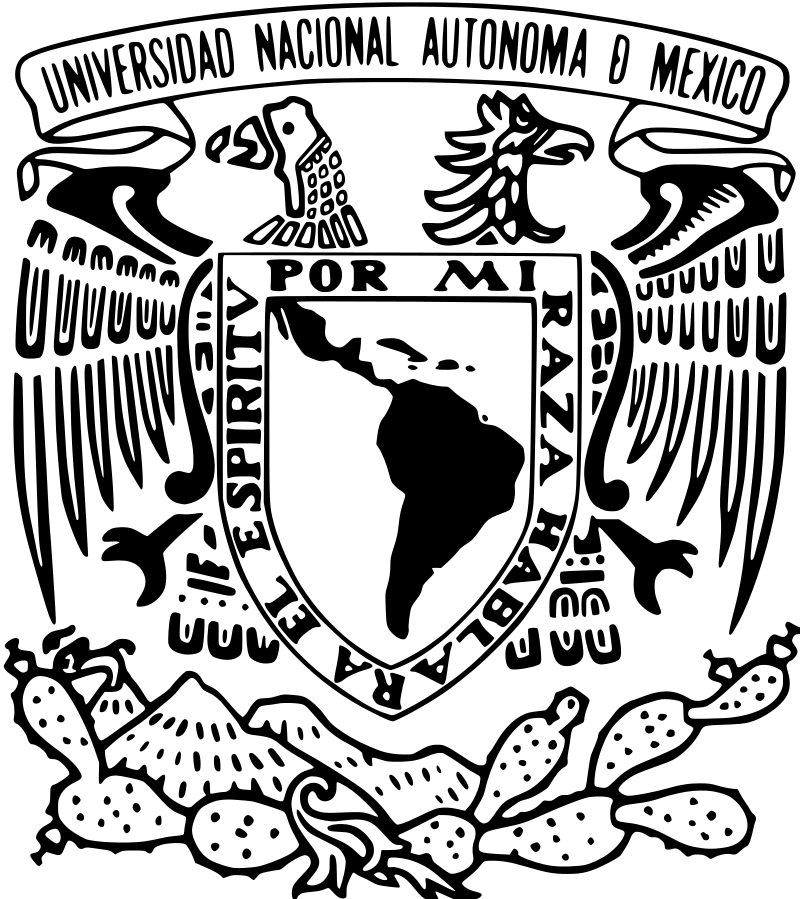
\includegraphics[width=4cm]{escudoUNAM.png}
		};

		\node[anchor=north east, inner sep=30] at (current page.north east) {
			
\includegraphics[width=4cm]{escudoFI.png}
		};
	\end{tikzpicture}

	\begin{center}
		\vspace*{3cm}

		\Huge
		\textbf{Practica 2 - Análisis Senoidal Permanente de Circuitos Lineales}

		\vspace{2.5cm}

		\Huge
		\textbf{Facultad de Ingeniería}\\
		Circuitos Eléctricos\\
		Semestre 2026-1\\

		\vspace{2.5cm}

		\textbf{Grupo:} 4

		\vspace{2.5cm}

		\Huge
		Ugartechea González Luis Antonio\\
		Tepal Brinseño Hansel Yael \\
		\textbf{Fecha de entrega:} 
		\vspace{2.5cm}
	\end{center}

\end{titlepage}

\section{Objetivo}

\begin{itemize}
	\item Verificar en forma práctica las técnicas de análisis senoidal permanente, empleando fasores.
\end{itemize}

\section{Marco Teórico}

\begin{itemize}
	\item \textbf{Fasor:} Representación compleja de una magnitud sinusoidal, utilizada en el análisis de circuitos eléctricos para simplificar cálculos.
	\item \textbf{Función de transferencia:} El cociente entre la transformada de Laplace de la salida y la transformada de Laplace de la entrada de un sistema, bajo la condición de que todas las condiciones iniciales sean cero.
\end{itemize}

\section{Desarrollo}

\subsection*{Circuito RL}

\begin{figure}[H]
	\centering
	\includegraphics
	\caption{Circuito RL}[width=0.5\textwidth]{figure_1.png}
\end{figure}

\subsubsection*{Función de Transferencia}

\[H(s) = \frac{R}{R_{eq} + sL}\]

\[H(j\omega) = \frac{R}{R_{eq} + j\omega L}\]

\subsubsection*{Obtención de ángulo de fase}

\[\Theta_Y = \angle Y(j\omega)\]

\[\Theta_X = \angle X(j\omega)\]

\[\Theta_Y = \tan^{-1}\left(\frac{\text{Im}(Y(j\omega))}{\text{Re}(Y(j\omega))}\right)\]

\[\Theta_X = \tan^{-1}\left(\frac{\text{Im}(X(j\omega))}{\text{Re}(X(j\omega))}\right)\]

\[\Theta_Y = \tan^{-1}\left(\frac{0}{R}\right)\]

\[\Theta_X = \tan^{-1}\left(\frac{\omega L}{R_{eq}}\right)\]

\[\Theta_H = \Theta_Y - \Theta_X\]

\subsubsection*{Magnitud de la señal}

\[
|H(j\omega)| = \frac{R}{\sqrt{R_{eq}^2 + (\omega L)^2}}
\]

\subsubsection*{Datos de Practica}

\begin{itemize}
	\item \textbf{Señal de entrada:} \(5 sen (\omega t)\)
	\item \textbf{\(\omega\):} \(4000 \pi \, rad/s\)
	\item \textbf{Frecuencia:} \(f = 2 kHz\)
	\item \textbf{Resistencia de la fuente:} \(50 \omega\)
	\item \textbf{Inductancia:} \(L =  72 mH\)
	\item \textbf{resistencia del inductor:} \(R_L = 72.7 \Omega\)
	\item \textbf{Resistencia:} \(R = 200 \Omega\)
\end{itemize}

\subsubsection*{Medidas prácticas}

\begin{itemize}
	\item \textbf{Ángulo de desfasamiento:} \(\Theta = \frac{1 [cuadro]\cdot (360°)}{5 [cuadros]} = 72°\)
	\item \textbf{Desfasamiento medido con cursor del osciloscopio:} \(71.2°\)
\end{itemize}

Despejamos \(L\):

\[
L = \frac{R_{eq}}{\omega} \cdot \tan(\Theta)
\]

Sustituimos para obtener \(L\):

\[
L = \frac{200 \Omega + 72.7 \Omega + 50 \Omega}{4000 \pi \, [\frac{rad}{s}]} \cdot \tan(72°) \approx 79.8 mH
\]

\textbf{Error porcentual:}

\[
\text{Error} = \left| \frac{L_{teorico} - L_{practico}}{L_{teorico}} \right| \cdot 100\%
\]
\[
\text{Error} = \left| \frac{79.8 mH - 72 mH}{72 mH} \right| \cdot 100\% \approx 10.83\%
\]

\subsection*{Circuito RC}

\begin{figure}[H]
	\centering
	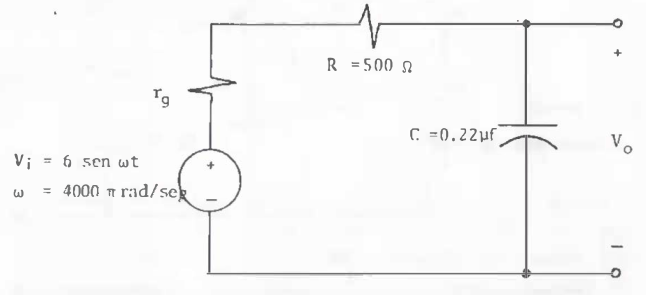
\includegraphics[width=0.6\textwidth]{figure_2.png}
	\caption{Circuito RC}
\end{figure}

\subsubsection*{Función de Transferencia}

\[H(s) = \frac{1}{1+sR_{eq}C}\]

\[H(j\omega) = \frac{1}{1+j\omega R_{eq}C}\]

\subsubsection*{Obtención de ángulo de fase}

\[\Theta_Y = \angle Y(j\omega)\]

\[\Theta_X = \angle X(j\omega)\]

\[\Theta_Y = \tan^{-1}\left(\frac{\text{Im}(Y(j\omega))}{\text{Re}(Y(j\omega))}\right)\]

\[\Theta_X = \tan^{-1}\left(\frac{\text{Im}(X(j\omega))}{\text{Re}(X(j\omega))}\right)\]

\[\Theta_H = \Theta_Y - \Theta_X\]

\[\Theta_H = \tan^{-1}\left(R_{eq}C\omega\right)\]

\[\Theta_H = \tan^{-1}\left((50\Omega +500[\Omega] )0.22[\mu F] 4000 \pi \, \left[\frac{rad}{s} \right] \right)\]

\[\Theta_H = 56.66°\]

\subsubsection*{Magnitud de la señal}

\[
|H(j\omega)| = \frac{1}{\sqrt{1 + (\omega R_{eq} C)^2}}
\]

\subsubsection*{Datos de Practica}

\begin{itemize}
	\item \textbf{Señal de entrada:} \(6 sen (\omega t)\)
	\item \textbf{\(\omega\):} \(4000 \pi \, rad/s\)
	\item \textbf{Frecuencia:} \(f = 2 kHz\)
	\item \textbf{Resistencia de la fuente:} \(50 \omega\)
	\item \textbf{Capacitancia:} \(C =  0.22 \mu F\)
	\item \textbf{Resistencia:} \(R = 500 \Omega\)
\end{itemize}

\subsubsection*{Medidas prácticas}

\begin{itemize}
	\item \textbf{Desfasamiento medido con cursor del osciloscopio:} \(56.1°\)
\end{itemize}

Despejamos \(C\):

\[
C = \frac{1}{\omega R_{eq}} \cdot \tan(\Theta)
\]

Sustituimos para obtener \(C\):

\[
C = \frac{1}{500 \Omega + 50 \Omega} \cdot \tan(56.1°) \approx 0.21 [\mu F]
\]

\textbf{Error porcentual:}

\[
\text{Error} = \left| \frac{C_{teorico} - C_{practico}}{C_{teorico}} \right| \cdot 100\%
\]
\[
\text{Error} = \left| \frac{0.22 [\mu F] - 0.21 [\mu F]}{0.22 [\mu F]} \right| \cdot 100\% \approx 4.54\%
\]

\subsection*{Circuito RC invertido}

\subsubsection*{Ángulo de fase}

\[
\Theta_H = \tan^{-1}\left(\frac{1}{R_{eq}C\omega}\right)
\]

\[
\Theta_H = \tan^{-1}\left(\frac{1}{(50\Omega + 500\Omega)0.22[\mu F] 4000 \pi \, \left[\frac{rad}{s} \right]}\right)
\]

\[
\Theta_H = 33.33°
\]

\subsubsection*{Datos de Practica}

\begin{itemize}
	\item \textbf{Señal de entrada:} \(6 sen (\omega t)\)
	\item \textbf{\(\omega\):} \(4000 \pi \, rad/s\)
	\item \textbf{Frecuencia:} \(f = 2 kHz\)
	\item \textbf{Resistencia de la fuente:} \(50 \Omega\)
	\item \textbf{Capacitancia:} \(C =  0.22 \mu F\)
	\item \textbf{Resistencia:} \(R = 500 \Omega\)
\end{itemize}

\subsubsection*{Medidas prácticas}

\begin{itemize}
	\item \textbf{Desfasamiento medido con cursor del osciloscopio:} \(36.8°\)
\end{itemize}

Despejamos \(C\):

\[
C = \frac{1}{R_{eq}\cdot \omega \cdot \tan(\Theta_H)}
\]

Sustituimos para obtener \(C\):

\[
C = \frac{1}{(50\Omega + 500\Omega) 4000 \pi \, \left[\frac{rad}{s} \right]\cdot \tan(36.8°)} \approx 0.19[\mu F]
\]

\textbf{Error porcentual:}

\[
\text{Error} = \left| \frac{C_{teorico} - C_{practico}}{C_{teorico}} \right| \cdot 100\%
\]
\[
\text{Error} = \left| \frac{0.22 [\mu F] - 0.19 [\mu F]}{0.22 [\mu F]} \right| \cdot 100\% \approx 15.78\%
\]

\subsubsection*{Observacion entre circuitos RC}

A diferencia del circuito anterior al colocar el capacitor primero vemos que ahora está adelanta con respecto a la señal de entrada.

\subsection*{Circuito RLC}

\begin{figure}[H]
	\centering
	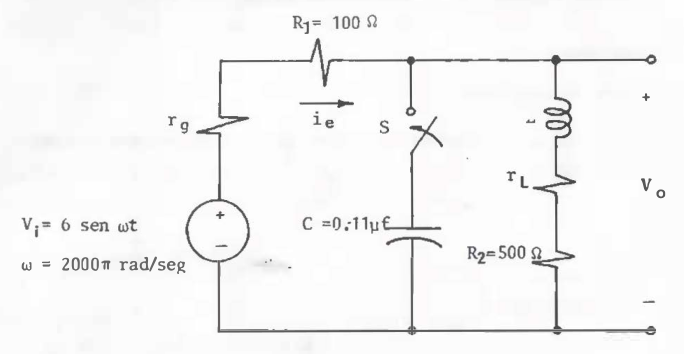
\includegraphics[width=0.6\textwidth]{figure_3.png}
	\caption{Circuito RLC}
\end{figure}

\subsubsection*{Ángulo de desfase}

\[
\Theta = \tan^{-1} \left(\frac{\omega C(r_L + R_2)}{1 -\omega LC} \right) - \tan^{-1}\left(\frac{\omega L}{r_L + R_2} \right)
\]

\[
\Theta = \tan^{-1} \left(\frac{(2000\pi)(0.11 \mu F)(72.7 \Omega + 500 \Omega)}{1 - (2000\pi)(0.11 \mu F)(72 mH)} \right) - \tan^{-1}\left(\frac{(2000\pi)(72 mH)}{72.7 \Omega + 500 \Omega} \right)
\]

\[
\Theta = 21.59° - 38.30° = -16.71°
\]


\subsubsection*{Datos de Practica}

\begin{itemize}
	\item \textbf{Señal de entrada:} \(6 sen (\omega t)\)
	\item \textbf{\(\omega\):} \(2000 \pi \, rad/s\)
	\item \textbf{Frecuencia:} \(f = 1 kHz\)
	\item \textbf{Resistencia de la fuente:} \(50 \Omega\)
	\item \textbf{Capacitancia:} \(C =  0.11 \mu F\)
	\item \textbf{Inductancia:} \(L =  72 mH\)
	\item \textbf{Resistencia del inductor:} \(R_L = 72.7 \Omega\)
	\item \textbf{Resistencia:} \(R_1 = 100 \Omega\)
	\item \textbf{Resistencia:} \(R_2 = 500 \Omega\)
\end{itemize}

\subsection*{Experimento 3}



% \section{Bibliography}

% \begin{biblio}
% 	%for: https://www.poli.edu.co/blog/poliverso/diseno-digital-que-es
% 	\item \textit{Diseño digital: qué es y por qué es importante.} (2021, August 26). Poliverso. Retrieved October 16, 2024, from: \textcolor{blue}{\underline{\url{https://www.poli.edu.co/blog/poliverso/diseno-digital-que-es}}}
% 	%for: https://www.sky6cancun.com/marketing/diseno-grafico/diseno-digital-que-es-y-para-que-sirve/
% 	\item \textit{Diseño digital: qué es y para qué sirve.} (2021, August 26). Sky6Cancún. Retrieved October 16, 2024, from: \textcolor{blue}{\underline{\url{https://www.sky6cancun.com/marketing/diseno-grafico/}}}
% \end{biblio}

\end{document}
